\epigraph{A theory without testable predictions is philosophy. T0 delivers numbers.}{}

A physical theory must be measured --- literally. The T0 theory makes a series of concrete, quantitative predictions that are verifiable with current or near-future technology.

\section{Bell Test Deviations}


\begin{figure}[htbp]
\centering
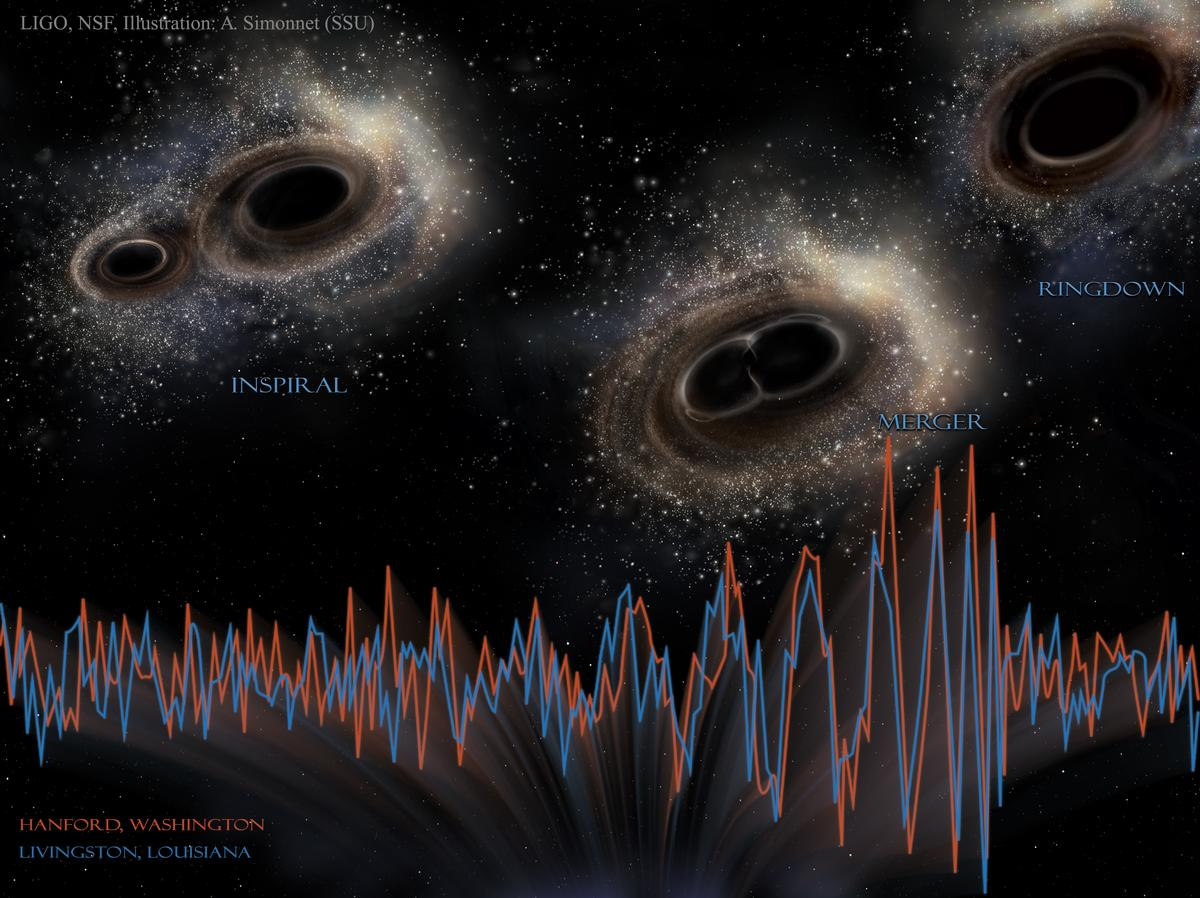
\includegraphics[width=0.85\textwidth]{img/ligo_gw_big.jpg}
\caption{GW150914 (LIGO): two merging black holes --- inspiral, merger, ringdown. T0 predicts corrections at high frequencies. Credit: LIGO, NSF; Illustration: A.~Simonnet (SSU).}
\end{figure}
The T0-modified Bell inequalities predict deviations of order~$\sim 10^{-3}$ in multi-qubit systems. The choice of 73~qubits as benchmark follows from the analysis in \href{https://github.com/jpascher/T0-Time-Mass-Duality/blob/main/2/pdf/142_Experimet-verschraenkung_De.pdf}{Doc.~142}: at this system size the cumulative $\xsi$ correction to the CHSH correlations becomes systematically measurable for the first time, while the system remains experimentally controllable.

\section{Spatial Correlation Delays}

Over large distances T0 predicts measurable delays in entanglement correlations. The estimate follows from $\Delta t \approx \xsi \cdot d/c$: for $d = 1000$~km this gives $\Delta t \approx 1.33 \times 10^{-4} \times 1000\,\text{km} / c \approx 445$~nanoseconds (\href{https://github.com/jpascher/T0-Time-Mass-Duality/blob/main/2/pdf/020_T0_QM-QFT-RT_De.pdf}{Doc.~020}). This would be detectable in a satellite experiment --- comparable to the Chinese Micius experiment but with higher time resolution.

\section{Quantum Computer Error Rates}

The T0 correction to quantum computer error rates is systematic:
\begin{equation}
\varepsilon_{\text{T0}} = \varepsilon_{\text{standard}} \cdot \left(1 - \xsi \cdot \frac{E_{\text{gate}}}{E_{\text{Planck}}}\right)
\end{equation}

The correction is tiny but \emph{systematic} --- it should manifest as a consistent deviation from standard predictions in large quantum circuits.

\section{Atom Interferometry}

The latest generation of atom interferometers reaches sensitivities that make T0 corrections accessible. The predicted phase shift is~$\sim 10^{-18}$~radians --- at the edge of the currently measurable but within reach of planned experiments.

\section{Gravitational Wave Corrections}

The LIGO/Virgo observatories measure gravitational waves with unprecedented precision. T0 predicts corrections in the wave signals at high frequencies (cf.\ \href{https://github.com/jpascher/T0-Time-Mass-Duality/blob/main/2/pdf/025_T0_Kosmologie_De.pdf}{Doc.~025}, \href{https://github.com/jpascher/T0-Time-Mass-Duality/blob/main/2/pdf/026_T0_Geometrische_Kosmologie_De.pdf}{026} for the cosmological predictions) --- where the fractal structure of spacetime makes itself most strongly felt.

\begin{figure}[htbp]
\centering
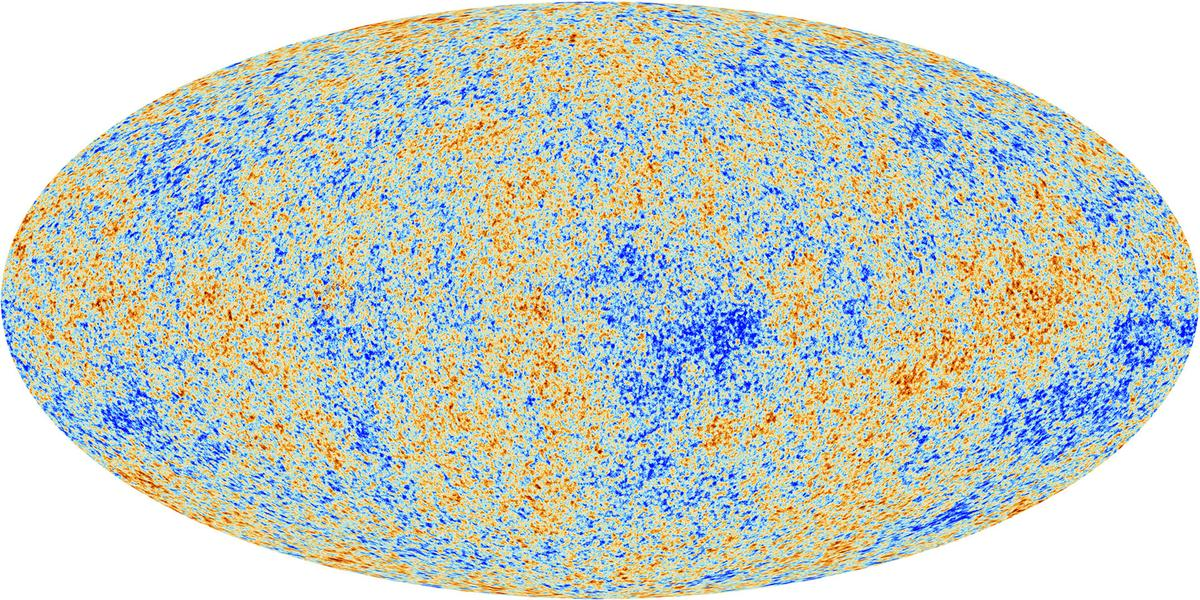
\includegraphics[width=\textwidth]{img/planck_cmb_final.jpg}
\caption{The cosmic microwave background radiation (CMB) as observed by the Planck satellite. In T0, the anisotropies arise from time-field variations --- not from inflationary expansion. Credit: ESA and the Planck Collaboration.}
\end{figure}

\section{The Tau Anomaly}

A particularly sharp prediction concerns the anomalous magnetic moment of the tau lepton:
\begin{equation}
a_\tau \approx 1.282 \times 10^{-3}
\end{equation}

This prediction is testable at the Belle~II experiment in Tsukuba, Japan. A confirmed value would be strong evidence for T0 geometry.

\begin{zusammenfassung}
T0 is not a purely theoretical construction. The theory makes at least half a dozen quantitative predictions verifiable with existing or planned experimental technology. Nature will decide.
\end{zusammenfassung}
